
\documentclass[11pt,a4paper,slovene]{article}

%Uporabljeni paketi
\usepackage[slovene]{babel}
\usepackage[utf8]{inputenc}
\usepackage{lmodern}
\usepackage[T1]{fontenc}
\usepackage{fancyhdr}
\usepackage{caption}
\captionsetup{font={default,footnotesize}, labelfont=bf, format=hang,indention=.0cm}
\usepackage{graphicx,epsfig}
\usepackage{amsmath}
\usepackage{multirow}
\usepackage{color}
\usepackage{url}
\usepackage{makeidx}
\usepackage[official]{eurosym}

\usepackage{hyperref}
\hypersetup{
   bookmarksnumbered=true,
   urlbordercolor={0 1 0},
   linkbordercolor={1 1 1},
   unicode=true,
   pdftitle={ Brezžična in Mobilna Omrežja },
   pdfauthor={Mojca Kompara},
   pdfdisplaydoctitle=true,
   pdftoolbar=true,
   pdfmenubar=true,
   pdfstartview=X Y Z
}

\urlstyle{same}

\setlength{\parskip}{12pt}
\setlength\parindent{0pt}
\setlength\unitlength{1mm}

\begin{document}
\label{naslov}
\pdfbookmark[1]{Naslov}{naslov}
\thispagestyle{empty}

\begin{center}
\begin{Large}
Brezžična in Mobilna Omrežja\\
Študijsko leto 2022/2023\\
\end{Large}

\vspace*{4cm}
\begin{LARGE}
\textbf{2. domača naloga\\}
\end{LARGE}
\vspace*{0.5cm}


\vspace*{4cm}

Mojca Kompara\\
Vpisna št. 63200147\\

\vspace*{5cm}
Ajdovščina, \today
\end{center}

\pagebreak
\setcounter{page}{1}
\pagenumbering{arabic}


\label{Kazalo}
\pdfbookmark[1]{Kazalo}{Kazalo}
\tableofcontents
\thispagestyle{empty}
\pagebreak

\section{Standard 802.11b}

Pri TCP protokolu je bila prepustnost povezave 9.07 Mbits/sec.
Pri UDP protokolu je bila prepustnost povezave 1.05 Mbits/sec in nihanje latence 0.997 ms.

\subsection{TCP protokol na Kali Linux}
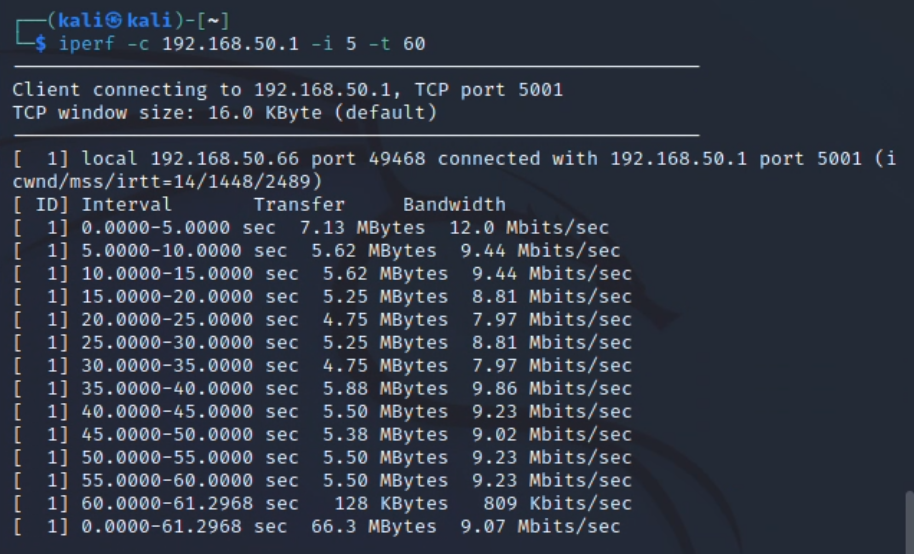
\includegraphics[width=\textwidth]{2_dn_tcp_b_kali}

\subsection{TCP protokol na Raspberry Pi}
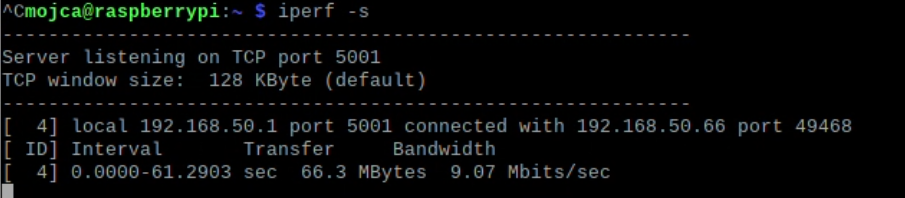
\includegraphics[width=\textwidth]{2_dn_tcp_b_rpi}

\subsection{UDP protokol na Kali Linux}
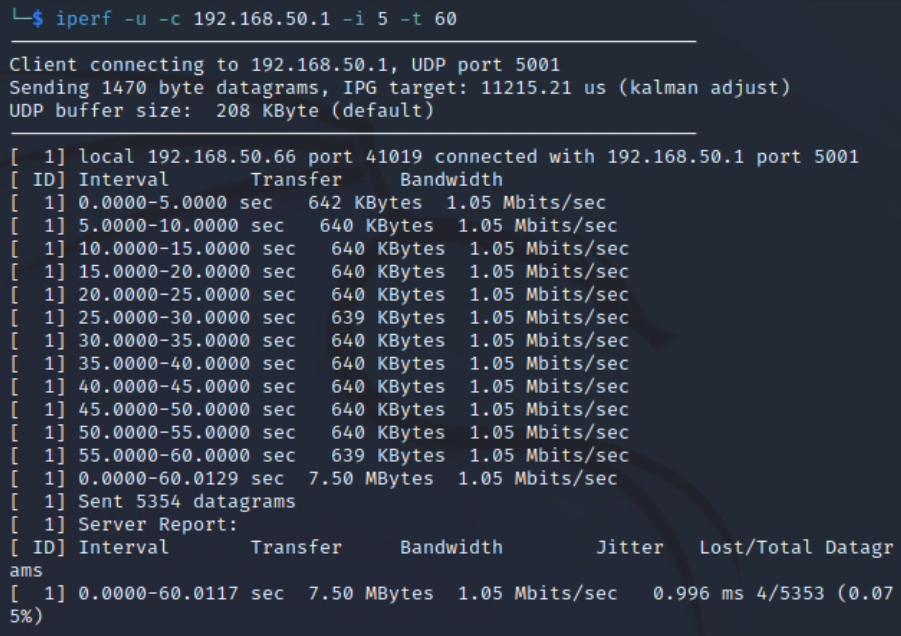
\includegraphics[width=\textwidth]{2_dn_udp_b_kali}

\subsection{UDP protokol na Raspberry Pi}
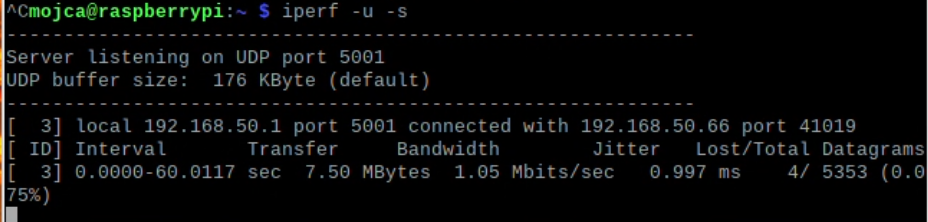
\includegraphics[width=\textwidth]{2_dn_udp_b_rpi}

\section{Standard 802.11g}

Pri TCP protokolu je bila prepustnost povezave 9.05 Mbits/sec.
Pri UDP protokolu je bila prepustnost povezave 1.05 Mbits/sec in nihanje latence 0.670 ms.

\subsection{TCP protokol na Kali Linux}
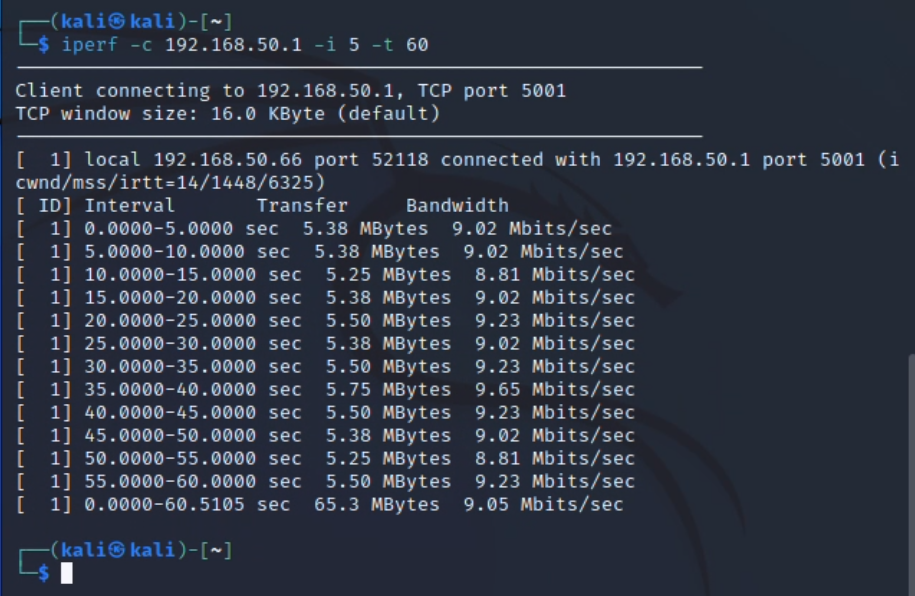
\includegraphics[width=\textwidth]{2_dn_tcp_g_kali}

\subsection{TCP protokol na Raspberry Pi}
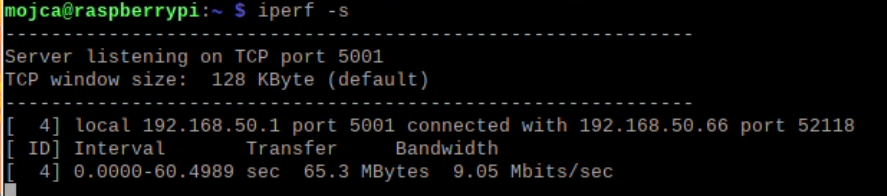
\includegraphics[width=\textwidth]{2_dn_tcp_g_rpi}

\subsection{UDP protokol na Kali Linux}
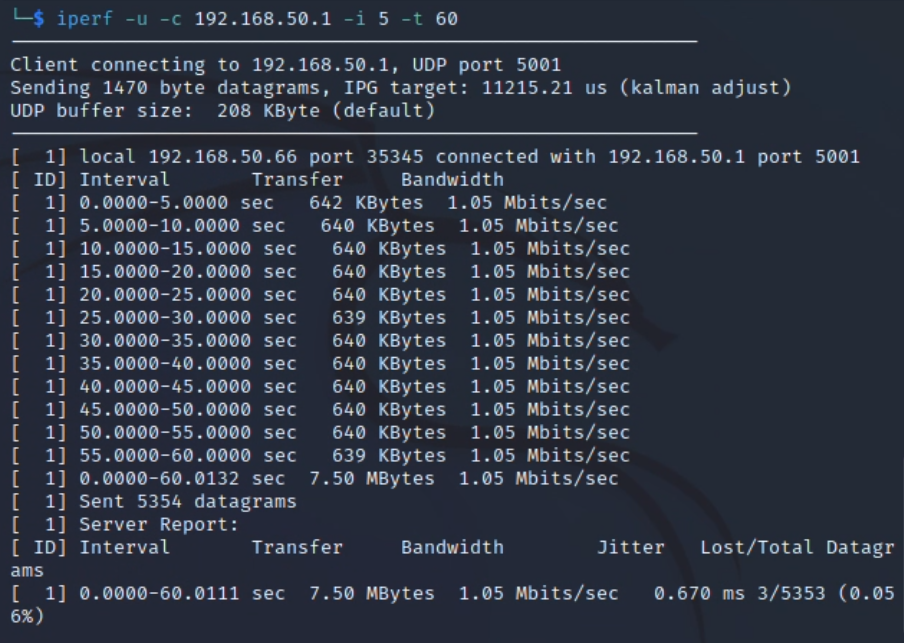
\includegraphics[width=\textwidth]{2_dn_udp_g_kali}

\subsection{UDP protokol na Raspberry Pi}
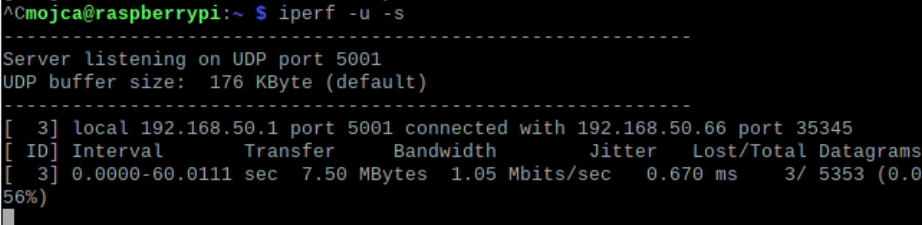
\includegraphics[width=\textwidth]{2_dn_udp_g_rpi}

\section{Konfiguracija RaspAP}
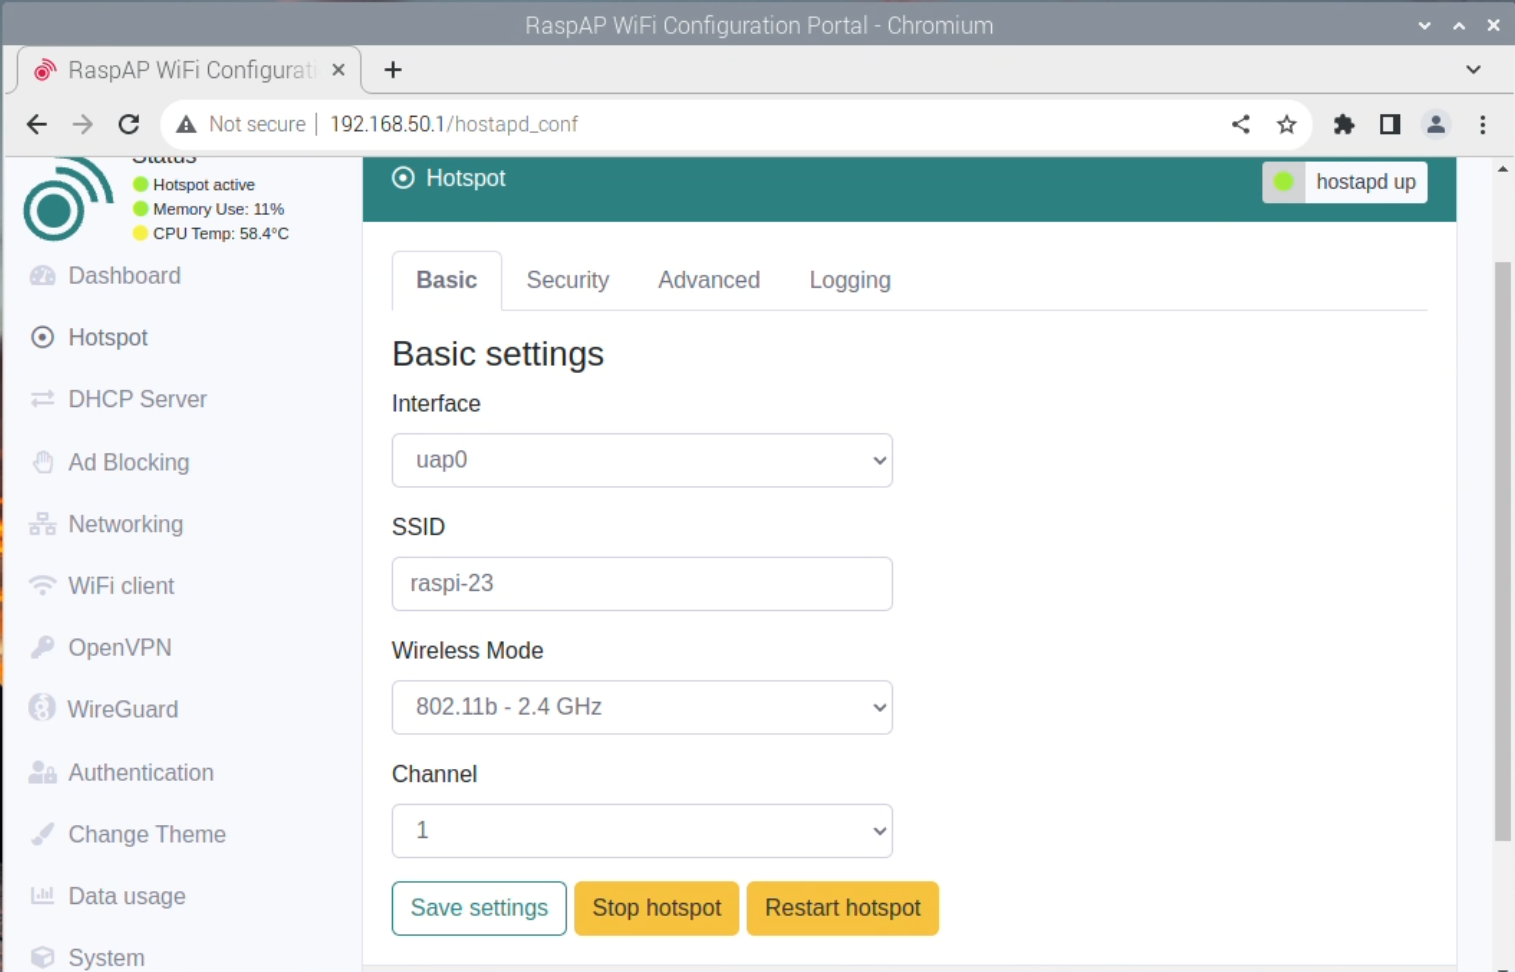
\includegraphics[width=\textwidth]{2_dn_raspapconf}


\pagebreak

\end{document}











